\documentclass[bachelor, och, labwork]{shiza}

\usepackage[utf8]{inputenc}
\usepackage{graphicx}

\usepackage[sort,compress]{cite}
\usepackage{amsmath}
\usepackage{amssymb}
\usepackage{amsthm}
\usepackage{fancyvrb}
\usepackage{longtable}
\usepackage{array}
\usepackage[english,russian]{babel}
\usepackage{minted}

\usepackage{tempora}


% \usepackage[colorlinks=false]{hyperref}


\newcommand{\eqdef}{\stackrel {\rm def}{=}}


\begin{document}

\title{Алгоритмы алгебры и теории чисел}

\course{4}

\group{431}

\napravlenie{10.05.01 "--- Компьютерная безопасность}


\author{Никитина Арсения Владимировича}


\satitle{доцент}
\saname{А.\,С.\,Гераськин}


\date{2022}

\maketitle

% Включение нумерации рисунков, формул и таблиц по разделам
% (по умолчанию - нумерация сквозная)
% (допускается оба вида нумерации)
%\secNumbering


\tableofcontents

\section{Задание лабораторной работы}

Реализовать алгоритмы вычисления НОД в кольцах полиномов:

\begin{enumerate}
    \item Расширенный алгоритм Евклида для полиномов над полем.
    \item Обобщённый алгоритм Евклида для полиномов над целыми числами.
\end{enumerate}

\section{Теоретическая часть}

\subsection{Расширенный алгоритм Евклида для полиномов над
полем (Extended Euclidean Algorithm for Polynomials over a Field)}


\textit{Вход:} $p_1(x), ~p_2(x) \in J[x], ~p_2(x) \not= 0, ~m = deg[p_1(x)] \geqslant deg[p_2(x)] = n$,
где $J$ --- поле.

\textit{Выход:} $p_(x), ~f(x), ~g(x) \in J[x]$, такие, что 
$deg[f(x)] < deg[p_1(x)] - deg[p_h(x)], ~deg[g(x)] < deg[p_2(x)] - deg[p_h(x)]$
и $p_h(x) = gcd[p_1(x), p_2(x)] = p_1(x)g(x) + p_2(x)f(x)$.


\begin{enumerate}
    \item Инициализировать переменные: 
    \begin{enumerate}
        \item $[p_0(x), p_1(x)] := [p_1(x), p_2(x)]$;
        \item $[g_0(x), g_1(x)] = [1, 0]$;
        \item $[f_0(x), f_1(x)] = [0, 1]$;
    \end{enumerate}
    \item Пока $p_1(x) \not= 0$:
    \begin{enumerate}
        \item $q(x) := \mathtt{PDF}[p_0(x), p_1(x)]$;
        \item $[p_0(x), p_1(x)] := [p_1(x), p_0(x) - p_1(x)q(x)]$;
        \item $[g_0(x), g_1(x)] := [g_1(x), g_0(x) - g_1(x)q(x)]$;
        \item $[f_0(x), f_1(x)] := [f_1(x), f_0(x) - f_1(x)q(x)]$;
    \end{enumerate}
    \item Вернуть $[p_h(x), g(x), f(x)] := [p_0(x), g_0(x), f_0(x)]$.
\end{enumerate}


\subsection{Обобщенный алгоритм Евклида для полиномов над це-
целыми числами (Generalized Euclidean Algorithm for Polynomials over
the Integers)}

\textit{Контент полинома (cont)} --- наибольший общий делитель всех коэффициентов
полинома.

\textit{Примитивная часть полинома (primitive part (pp))} --- исходный полином,
разделенный на его контент.

Полином также называют примитивным, если его контент равен единице, так как
примитивная часть полинома в данном случае будет являться исходным полиномом.

\textit{Вход:} $p_1(x), p_2(x)$ --- ненулевые полиномы в $\mathbb{Z}[x];$
$deg[p_1(x)] = n_1, deg[p_2(x)] = n_2, ~ n_1 \geqslant n_2.$

\textit{Выход:} $gcd[p_1(x), p_2(x)]$, НОД полиномов $p_1(x)$ и $p_2(x)$.

\begin{enumerate}
    
    \item Вычислить содержания gcd. Для этого перемнной $c$ присвоить значение
    $gcd(cont[p_1(x)], cont[p_2(x)])$.

    \item Вычислить примитивные части полиномов:
    \begin{enumerate}
        \item $p^{'}_1(x) = p_1(x) / cont[p_1(x)]$;
        \item $p^{'}_2(x) = p_2(x) / cont[p_2(x)]$;
    \end{enumerate}
    \item Построить PRS. Для этого выполнить последовательное деление полиномов
    в кольце целых чисел. Пока остаток в PDF не равен нулю:
    \begin{enumerate}
        \item $p_1(x), p_2(x) = p2(x), \mathtt{pdf}(p_1(x), p2(x))$.
    \end{enumerate}
    \item Если $deg[p_h(x)] = 0$ (предпоследний остаток от деления многочленов),
    то вернуть в качестве ответа $c$, иначе вернуть в качестве ответа
    $c\cdot pp[p_h(x)]$.
\end{enumerate}

\section{Практическая часть}
\subsection{Пример работы алгоритма}
\begin{figure}[H]
    \centering
    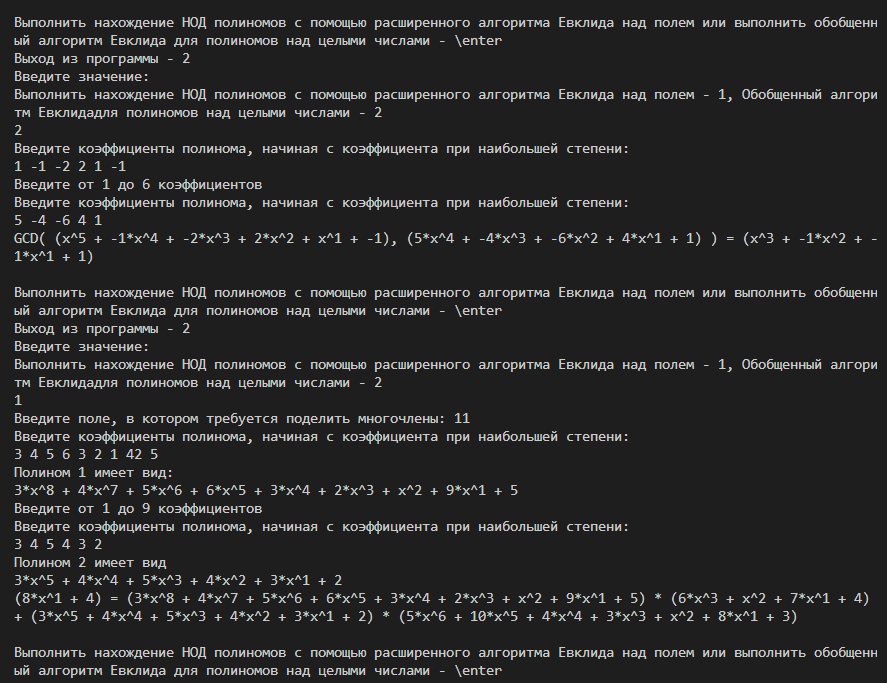
\includegraphics[width=1\textwidth]{pic1.png}
    \caption{}
\end{figure}

\setminted[python]{linenos,breaklines=true, fontsize=\small, style=bw}
    \subsection{Код программы, реализующей рассмотренный алгоритм}
        \inputminted{python}{lab14.py}


\end{document}